\documentclass[1p]{elsarticle_modified}
%\bibliographystyle{elsarticle-num}

%\usepackage[colorlinks]{hyperref}
%\usepackage{abbrmath_seonhwa} %\Abb, \Ascr, \Acal ,\Abf, \Afrak
\usepackage{amsfonts}
\usepackage{amssymb}
\usepackage{amsmath}
\usepackage{amsthm}
\usepackage{scalefnt}
\usepackage{amsbsy}
\usepackage{kotex}
\usepackage{caption}
\usepackage{subfig}
\usepackage{color}
\usepackage{graphicx}
\usepackage{xcolor} %% white, black, red, green, blue, cyan, magenta, yellow
\usepackage{float}
\usepackage{setspace}
\usepackage{hyperref}

\usepackage{tikz}
\usetikzlibrary{arrows}

\usepackage{multirow}
\usepackage{array} % fixed length table
\usepackage{hhline}

%%%%%%%%%%%%%%%%%%%%%
\makeatletter
\renewcommand*\env@matrix[1][\arraystretch]{%
	\edef\arraystretch{#1}%
	\hskip -\arraycolsep
	\let\@ifnextchar\new@ifnextchar
	\array{*\c@MaxMatrixCols c}}
\makeatother %https://tex.stackexchange.com/questions/14071/how-can-i-increase-the-line-spacing-in-a-matrix
%%%%%%%%%%%%%%%

\usepackage[normalem]{ulem}

\newcommand{\msout}[1]{\ifmmode\text{\sout{\ensuremath{#1}}}\else\sout{#1}\fi}
%SOURCE: \msout is \stkout macro in https://tex.stackexchange.com/questions/20609/strikeout-in-math-mode

\newcommand{\cancel}[1]{
	\ifmmode
	{\color{red}\msout{#1}}
	\else
	{\color{red}\sout{#1}}
	\fi
}

\newcommand{\add}[1]{
	{\color{blue}\uwave{#1}}
}

\newcommand{\replace}[2]{
	\ifmmode
	{\color{red}\msout{#1}}{\color{blue}\uwave{#2}}
	\else
	{\color{red}\sout{#1}}{\color{blue}\uwave{#2}}
	\fi
}

\newcommand{\Sol}{\mathcal{S}} %segment
\newcommand{\D}{D} %diagram
\newcommand{\A}{\mathcal{A}} %arc


%%%%%%%%%%%%%%%%%%%%%%%%%%%%%5 test

\def\sl{\operatorname{\textup{SL}}(2,\Cbb)}
\def\psl{\operatorname{\textup{PSL}}(2,\Cbb)}
\def\quan{\mkern 1mu \triangleright \mkern 1mu}

\theoremstyle{definition}
\newtheorem{thm}{Theorem}[section]
\newtheorem{prop}[thm]{Proposition}
\newtheorem{lem}[thm]{Lemma}
\newtheorem{ques}[thm]{Question}
\newtheorem{cor}[thm]{Corollary}
\newtheorem{defn}[thm]{Definition}
\newtheorem{exam}[thm]{Example}
\newtheorem{rmk}[thm]{Remark}
\newtheorem{alg}[thm]{Algorithm}

\newcommand{\I}{\sqrt{-1}}
\begin{document}

%\begin{frontmatter}
%
%\title{Boundary parabolic representations of knots up to 8 crossings}
%
%%% Group authors per affiliation:
%\author{Yunhi Cho} 
%\address{Department of Mathematics, University of Seoul, Seoul, Korea}
%\ead{yhcho@uos.ac.kr}
%
%
%\author{Seonhwa Kim} %\fnref{s_kim}}
%\address{Center for Geometry and Physics, Institute for Basic Science, Pohang, 37673, Korea}
%\ead{ryeona17@ibs.re.kr}
%
%\author{Hyuk Kim}
%\address{Department of Mathematical Sciences, Seoul National University, Seoul 08826, Korea}
%\ead{hyukkim@snu.ac.kr}
%
%\author{Seokbeom Yoon}
%\address{Department of Mathematical Sciences, Seoul National University, Seoul, 08826,  Korea}
%\ead{sbyoon15@snu.ac.kr}
%
%\begin{abstract}
%We find all boundary parabolic representation of knots up to 8 crossings.
%
%\end{abstract}
%\begin{keyword}
%    \MSC[2010] 57M25 
%\end{keyword}
%
%\end{frontmatter}

%\linenumbers
%\tableofcontents
%
\newcommand\colored[1]{\textcolor{white}{\rule[-0.35ex]{0.8em}{1.4ex}}\kern-0.8em\color{red} #1}%
%\newcommand\colored[1]{\textcolor{white}{ #1}\kern-2.17ex	\textcolor{white}{ #1}\kern-1.81ex	\textcolor{white}{ #1}\kern-2.15ex\color{red}#1	}

{\Large $\underline{10_{102}~(K10a_{97})}$}

\setlength{\tabcolsep}{10pt}
\renewcommand{\arraystretch}{1.6}
\vspace{1cm}\begin{tabular}{m{100pt}>{\centering\arraybackslash}m{274pt}}
\multirow{5}{120pt}{
	\centering
	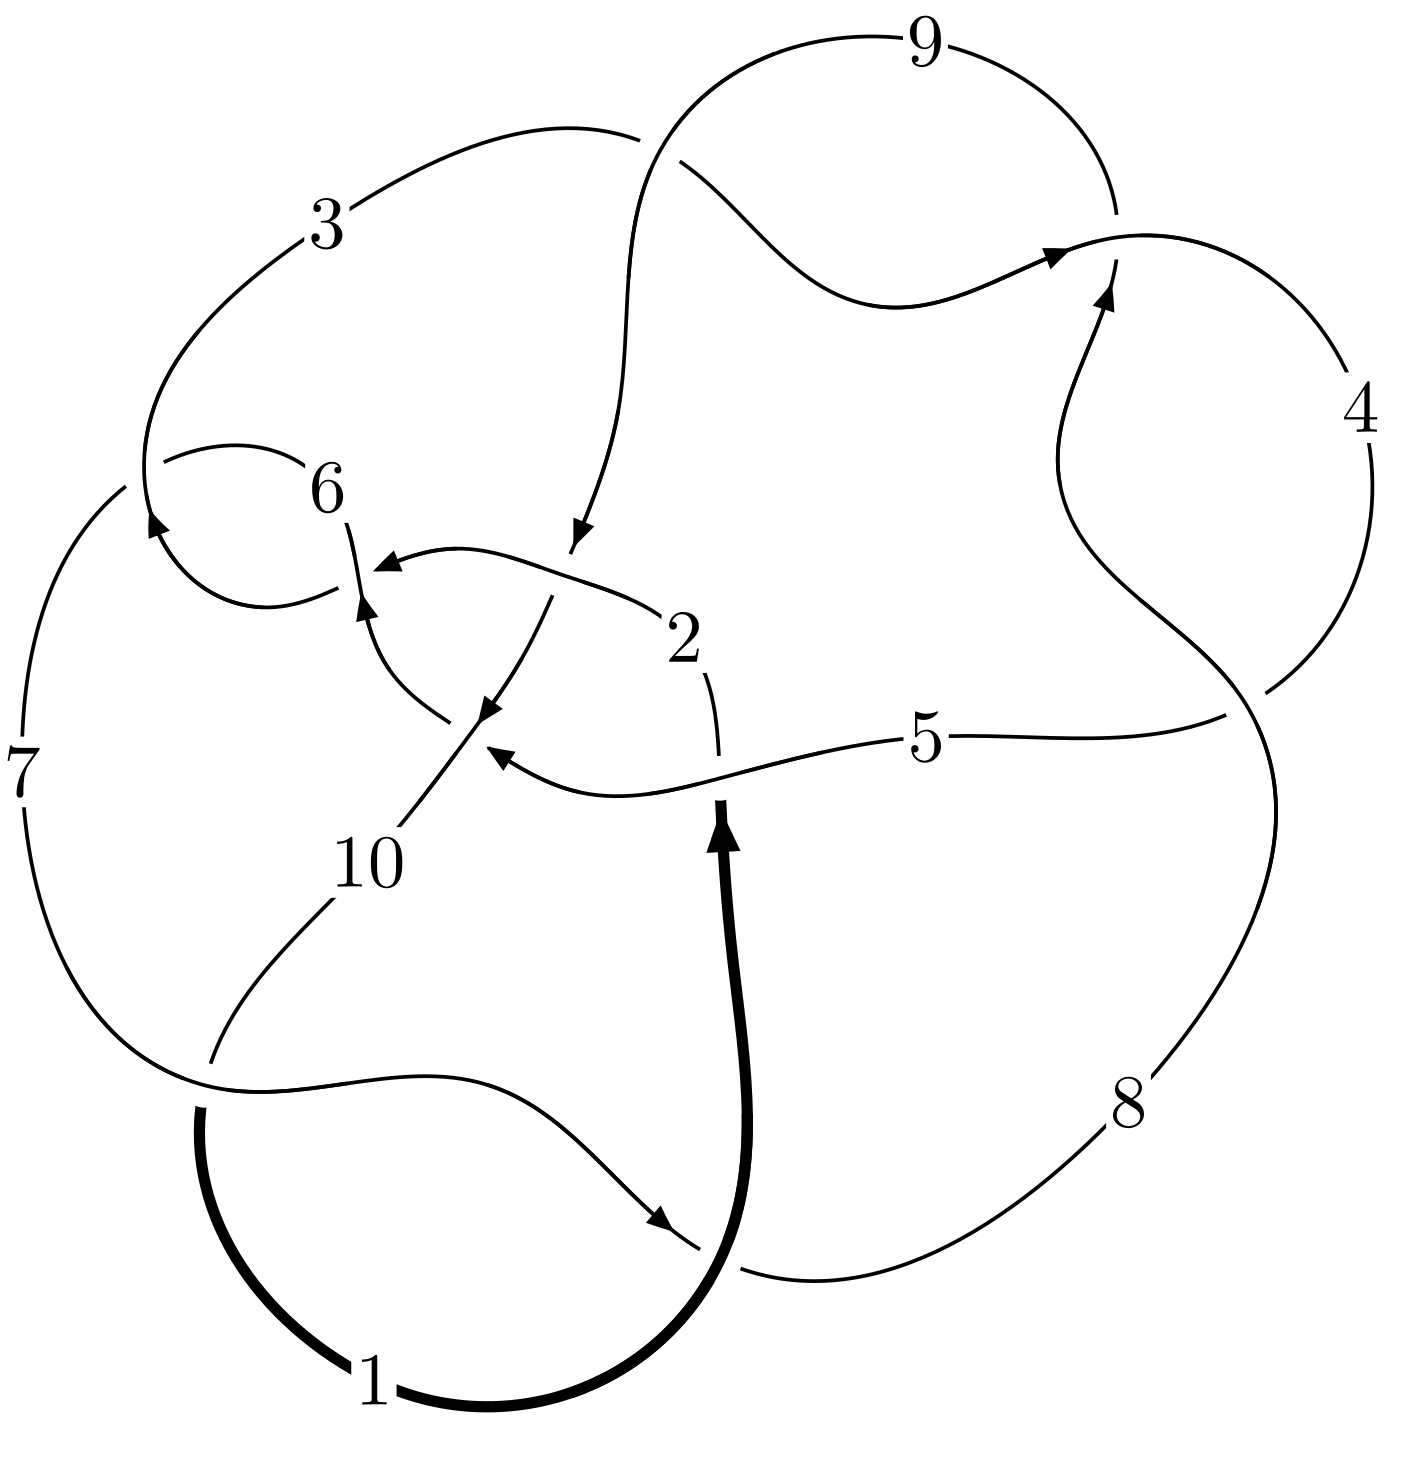
\includegraphics[width=112pt]{../../../GIT/diagram.site/Diagrams/png/186_10_102.png}\\
\ \ \ A knot diagram\footnotemark}&
\allowdisplaybreaks
\textbf{Linearized knot diagam} \\
\cline{2-2}
 &
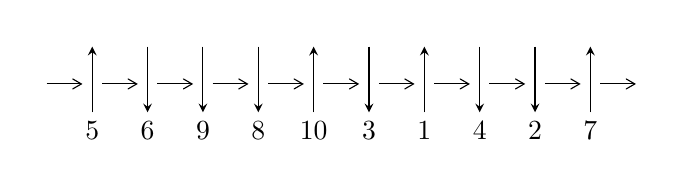
\begin{tikzpicture}[x=20pt, y=17pt]
	% nodes
	\node (C0) at (0, 0) {};
	\node (C1) at (1, 0) {};
	\node (C1U) at (1, +1) {};
	\node (C1D) at (1, -1) {5};

	\node (C2) at (2, 0) {};
	\node (C2U) at (2, +1) {};
	\node (C2D) at (2, -1) {6};

	\node (C3) at (3, 0) {};
	\node (C3U) at (3, +1) {};
	\node (C3D) at (3, -1) {9};

	\node (C4) at (4, 0) {};
	\node (C4U) at (4, +1) {};
	\node (C4D) at (4, -1) {8};

	\node (C5) at (5, 0) {};
	\node (C5U) at (5, +1) {};
	\node (C5D) at (5, -1) {10};

	\node (C6) at (6, 0) {};
	\node (C6U) at (6, +1) {};
	\node (C6D) at (6, -1) {3};

	\node (C7) at (7, 0) {};
	\node (C7U) at (7, +1) {};
	\node (C7D) at (7, -1) {1};

	\node (C8) at (8, 0) {};
	\node (C8U) at (8, +1) {};
	\node (C8D) at (8, -1) {4};

	\node (C9) at (9, 0) {};
	\node (C9U) at (9, +1) {};
	\node (C9D) at (9, -1) {2};

	\node (C10) at (10, 0) {};
	\node (C10U) at (10, +1) {};
	\node (C10D) at (10, -1) {7};
	\node (C11) at (11, 0) {};

	% arrows
	\draw[->,>={angle 60}]
	(C0) edge (C1) (C1) edge (C2) (C2) edge (C3) (C3) edge (C4) (C4) edge (C5) (C5) edge (C6) (C6) edge (C7) (C7) edge (C8) (C8) edge (C9) (C9) edge (C10) (C10) edge (C11) ;	\draw[->,>=stealth]
	(C1D) edge (C1U) (C2U) edge (C2D) (C3U) edge (C3D) (C4U) edge (C4D) (C5D) edge (C5U) (C6U) edge (C6D) (C7D) edge (C7U) (C8U) edge (C8D) (C9U) edge (C9D) (C10D) edge (C10U) ;
	\end{tikzpicture} \\
\hhline{~~} \\& 
\textbf{Solving Sequence} \\ \cline{2-2} 
 &
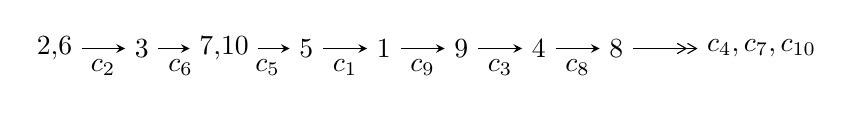
\begin{tikzpicture}[x=28pt, y=7pt]
	% node
	\node (A0) at (-1/8, 0) {2,6};
	\node (A1) at (1, 0) {3};
	\node (A2) at (33/16, 0) {7,10};
	\node (A3) at (25/8, 0) {5};
	\node (A4) at (33/8, 0) {1};
	\node (A5) at (41/8, 0) {9};
	\node (A6) at (49/8, 0) {4};
	\node (A7) at (57/8, 0) {8};
	\node (C1) at (1/2, -1) {$c_{2}$};
	\node (C2) at (3/2, -1) {$c_{6}$};
	\node (C3) at (21/8, -1) {$c_{5}$};
	\node (C4) at (29/8, -1) {$c_{1}$};
	\node (C5) at (37/8, -1) {$c_{9}$};
	\node (C6) at (45/8, -1) {$c_{3}$};
	\node (C7) at (53/8, -1) {$c_{8}$};
	\node (A8) at (9, 0) {$c_{4},c_{7},c_{10}$};

	% edge
	\draw[->,>=stealth]	
	(A0) edge (A1) (A1) edge (A2) (A2) edge (A3) (A3) edge (A4) (A4) edge (A5) (A5) edge (A6) (A6) edge (A7) ;
	\draw[->>,>={angle 60}]	
	(A7) edge (A8);
\end{tikzpicture} \\ 

\end{tabular} \\

\footnotetext{
The image of knot diagram is generated by the software ``\textbf{Draw programme}" developed by Andrew Bartholomew(\url{http://www.layer8.co.uk/maths/draw/index.htm\#Running-draw}), where we modified some parts for our purpose(\url{https://github.com/CATsTAILs/LinksPainter}).
}\phantom \\ \newline 
\centering \textbf{Ideals for irreducible components\footnotemark of $X_{\text{par}}$} 
 
\begin{align*}
I^u_{1}&=\langle 
-2.25484\times10^{39} u^{42}+2.20978\times10^{39} u^{41}+\cdots+2.97870\times10^{39} b-1.19885\times10^{39},\\
\phantom{I^u_{1}}&\phantom{= \langle  }-3.16887\times10^{39} u^{42}-4.11086\times10^{36} u^{41}+\cdots+2.97870\times10^{39} a+2.58687\times10^{40},\\
\phantom{I^u_{1}}&\phantom{= \langle  }u^{43}-12 u^{41}+\cdots-7 u-1\rangle \\
I^u_{2}&=\langle 
u^6-3 u^4- u^3+6 u^2+b-3,\;- u^6- u^5+u^4+2 u^3-2 u^2+a- u-1,\;u^7+u^6-2 u^5-3 u^4+3 u^3+3 u^2- u-1\rangle \\
\\
\end{align*}
\raggedright * 2 irreducible components of $\dim_{\mathbb{C}}=0$, with total 50 representations.\\
\footnotetext{All coefficients of polynomials are rational numbers. But the coefficients are sometimes approximated in decimal forms when there is not enough margin.}
\newpage
\renewcommand{\arraystretch}{1}
\centering \section*{I. $I^u_{1}= \langle -2.25\times10^{39} u^{42}+2.21\times10^{39} u^{41}+\cdots+2.98\times10^{39} b-1.20\times10^{39},\;-3.17\times10^{39} u^{42}-4.11\times10^{36} u^{41}+\cdots+2.98\times10^{39} a+2.59\times10^{40},\;u^{43}-12 u^{41}+\cdots-7 u-1 \rangle$}
\flushleft \textbf{(i) Arc colorings}\\
\begin{tabular}{m{7pt} m{180pt} m{7pt} m{180pt} }
\flushright $a_{2}=$&$\begin{pmatrix}1\\0\end{pmatrix}$ \\
\flushright $a_{6}=$&$\begin{pmatrix}0\\u\end{pmatrix}$ \\
\flushright $a_{3}=$&$\begin{pmatrix}1\\u^2\end{pmatrix}$ \\
\flushright $a_{7}=$&$\begin{pmatrix}- u\\- u^3+u\end{pmatrix}$ \\
\flushright $a_{10}=$&$\begin{pmatrix}1.06384 u^{42}+0.00138009 u^{41}+\cdots-8.11372 u-8.68458\\0.756988 u^{42}-0.741862 u^{41}+\cdots-0.408776 u+0.402477\end{pmatrix}$ \\
\flushright $a_{5}=$&$\begin{pmatrix}-0.534324 u^{42}-0.672258 u^{41}+\cdots+3.56812 u+10.8345\\-0.489904 u^{42}+0.404335 u^{41}+\cdots+3.17936 u-0.269339\end{pmatrix}$ \\
\flushright $a_{1}=$&$\begin{pmatrix}1.67244 u^{42}-0.522788 u^{41}+\cdots-8.92616 u-9.02482\\0.644047 u^{42}-0.551896 u^{41}+\cdots-2.65691 u+0.218556\end{pmatrix}$ \\
\flushright $a_{9}=$&$\begin{pmatrix}1.82083 u^{42}-0.740482 u^{41}+\cdots-8.52249 u-8.28210\\0.756988 u^{42}-0.741862 u^{41}+\cdots-0.408776 u+0.402477\end{pmatrix}$ \\
\flushright $a_{4}=$&$\begin{pmatrix}-0.891489 u^{42}+1.06089 u^{41}+\cdots+7.38092 u-2.51083\\-0.892905 u^{42}+0.445547 u^{41}+\cdots+7.63273 u+1.57813\end{pmatrix}$ \\
\flushright $a_{8}=$&$\begin{pmatrix}0.580848 u^{42}+1.18966 u^{41}+\cdots-4.91202 u-10.4146\\-0.291565 u^{42}+0.524997 u^{41}+\cdots+0.716241 u+0.694269\end{pmatrix}$\\&\end{tabular}
\flushleft \textbf{(ii) Obstruction class $= -1$}\\~\\
\flushleft \textbf{(iii) Cusp Shapes $= 3.56001 u^{42}-2.01639 u^{41}+\cdots-29.9474 u-1.29868$}\\~\\
\newpage\renewcommand{\arraystretch}{1}
\flushleft \textbf{(iv) u-Polynomials at the component}\newline \\
\begin{tabular}{m{50pt}|m{274pt}}
Crossings & \hspace{64pt}u-Polynomials at each crossing \\
\hline $$\begin{aligned}c_{1}\end{aligned}$$&$\begin{aligned}
&u^{43}-3 u^{42}+\cdots-1000 u+419
\end{aligned}$\\
\hline $$\begin{aligned}c_{2},c_{6}\end{aligned}$$&$\begin{aligned}
&u^{43}-12 u^{41}+\cdots-7 u-1
\end{aligned}$\\
\hline $$\begin{aligned}c_{3},c_{4},c_{8}\end{aligned}$$&$\begin{aligned}
&u^{43}+u^{42}+\cdots+10 u-1
\end{aligned}$\\
\hline $$\begin{aligned}c_{5}\end{aligned}$$&$\begin{aligned}
&u^{43}+u^{42}+\cdots+2 u-1
\end{aligned}$\\
\hline $$\begin{aligned}c_{7},c_{10}\end{aligned}$$&$\begin{aligned}
&u^{43}-17 u^{41}+\cdots+85 u-19
\end{aligned}$\\
\hline $$\begin{aligned}c_{9}\end{aligned}$$&$\begin{aligned}
&u^{43}-7 u^{42}+\cdots+18 u-1
\end{aligned}$\\
\hline
\end{tabular}\\~\\
\newpage\renewcommand{\arraystretch}{1}
\flushleft \textbf{(v) Riley Polynomials at the component}\newline \\
\begin{tabular}{m{50pt}|m{274pt}}
Crossings & \hspace{64pt}Riley Polynomials at each crossing \\
\hline $$\begin{aligned}c_{1}\end{aligned}$$&$\begin{aligned}
&y^{43}-17 y^{42}+\cdots+2566222 y-175561
\end{aligned}$\\
\hline $$\begin{aligned}c_{2},c_{6}\end{aligned}$$&$\begin{aligned}
&y^{43}-24 y^{42}+\cdots+29 y-1
\end{aligned}$\\
\hline $$\begin{aligned}c_{3},c_{4},c_{8}\end{aligned}$$&$\begin{aligned}
&y^{43}+45 y^{42}+\cdots+28 y-1
\end{aligned}$\\
\hline $$\begin{aligned}c_{5}\end{aligned}$$&$\begin{aligned}
&y^{43}+y^{42}+\cdots+8 y-1
\end{aligned}$\\
\hline $$\begin{aligned}c_{7},c_{10}\end{aligned}$$&$\begin{aligned}
&y^{43}-34 y^{42}+\cdots+4299 y-361
\end{aligned}$\\
\hline $$\begin{aligned}c_{9}\end{aligned}$$&$\begin{aligned}
&y^{43}+y^{42}+\cdots+68 y-1
\end{aligned}$\\
\hline
\end{tabular}\\~\\
\newpage\flushleft \textbf{(vi) Complex Volumes and Cusp Shapes}
$$\begin{array}{c|c|c}  
\text{Solutions to }I^u_{1}& \I (\text{vol} + \sqrt{-1}CS) & \text{Cusp shape}\\
 \hline 
\begin{aligned}
u &= \phantom{-}0.179428 + 0.966528 I \\
a &= -0.758038 + 0.845663 I \\
b &= \phantom{-}0.655485 - 0.701109 I\end{aligned}
 & \phantom{-}3.68686 + 3.98038 I & \phantom{-}2.52488 - 5.84737 I \\ \hline\begin{aligned}
u &= \phantom{-}0.179428 - 0.966528 I \\
a &= -0.758038 - 0.845663 I \\
b &= \phantom{-}0.655485 + 0.701109 I\end{aligned}
 & \phantom{-}3.68686 - 3.98038 I & \phantom{-}2.52488 + 5.84737 I \\ \hline\begin{aligned}
u &= \phantom{-}0.873967 + 0.439410 I \\
a &= -1.86520 - 0.23703 I \\
b &= -0.248002 - 0.538074 I\end{aligned}
 & \phantom{-}8.42806 - 4.73173 I & \phantom{-}3.14920 + 6.15524 I \\ \hline\begin{aligned}
u &= \phantom{-}0.873967 - 0.439410 I \\
a &= -1.86520 + 0.23703 I \\
b &= -0.248002 + 0.538074 I\end{aligned}
 & \phantom{-}8.42806 + 4.73173 I & \phantom{-}3.14920 - 6.15524 I \\ \hline\begin{aligned}
u &= -0.894503 + 0.382311 I \\
a &= \phantom{-}1.176590 + 0.347821 I \\
b &= \phantom{-}1.61995 - 0.69095 I\end{aligned}
 & \phantom{-}8.00794 - 0.59552 I & \phantom{-}3.42142 - 0.64701 I \\ \hline\begin{aligned}
u &= -0.894503 - 0.382311 I \\
a &= \phantom{-}1.176590 - 0.347821 I \\
b &= \phantom{-}1.61995 + 0.69095 I\end{aligned}
 & \phantom{-}8.00794 + 0.59552 I & \phantom{-}3.42142 + 0.64701 I \\ \hline\begin{aligned}
u &= -0.937588 + 0.179486 I \\
a &= -0.339877 - 1.370130 I \\
b &= -0.908003 + 0.652924 I\end{aligned}
 & -1.78551 + 0.79823 I & -3.86305 + 0.92711 I \\ \hline\begin{aligned}
u &= -0.937588 - 0.179486 I \\
a &= -0.339877 + 1.370130 I \\
b &= -0.908003 - 0.652924 I\end{aligned}
 & -1.78551 - 0.79823 I & -3.86305 - 0.92711 I \\ \hline\begin{aligned}
u &= \phantom{-}1.005980 + 0.308159 I \\
a &= -0.113439 + 0.394153 I \\
b &= \phantom{-}0.524877 - 0.944675 I\end{aligned}
 & \phantom{-}0.85124 - 2.72416 I & \phantom{-}2.00505 + 5.61413 I \\ \hline\begin{aligned}
u &= \phantom{-}1.005980 - 0.308159 I \\
a &= -0.113439 - 0.394153 I \\
b &= \phantom{-}0.524877 + 0.944675 I\end{aligned}
 & \phantom{-}0.85124 + 2.72416 I & \phantom{-}2.00505 - 5.61413 I\\
 \hline 
 \end{array}$$\newpage$$\begin{array}{c|c|c}  
\text{Solutions to }I^u_{1}& \I (\text{vol} + \sqrt{-1}CS) & \text{Cusp shape}\\
 \hline 
\begin{aligned}
u &= \phantom{-}0.765516 + 0.410276 I \\
a &= -0.11829 - 1.69787 I \\
b &= -0.114903 + 1.388430 I\end{aligned}
 & \phantom{-}8.79687 + 1.11797 I & \phantom{-}3.28924 + 1.64001 I \\ \hline\begin{aligned}
u &= \phantom{-}0.765516 - 0.410276 I \\
a &= -0.11829 + 1.69787 I \\
b &= -0.114903 - 1.388430 I\end{aligned}
 & \phantom{-}8.79687 - 1.11797 I & \phantom{-}3.28924 - 1.64001 I \\ \hline\begin{aligned}
u &= -0.028174 + 0.866113 I \\
a &= \phantom{-}0.809304 + 0.674158 I \\
b &= -0.391438 - 1.141660 I\end{aligned}
 & \phantom{-}6.04283 - 2.22576 I & \phantom{-}2.85072 + 2.97682 I \\ \hline\begin{aligned}
u &= -0.028174 - 0.866113 I \\
a &= \phantom{-}0.809304 - 0.674158 I \\
b &= -0.391438 + 1.141660 I\end{aligned}
 & \phantom{-}6.04283 + 2.22576 I & \phantom{-}2.85072 - 2.97682 I \\ \hline\begin{aligned}
u &= -0.780496 + 0.342696 I \\
a &= -0.346122 - 0.358729 I \\
b &= \phantom{-}1.14579 + 1.89719 I\end{aligned}
 & \phantom{-}8.42175 + 3.77684 I & \phantom{-}3.65503 - 8.57155 I \\ \hline\begin{aligned}
u &= -0.780496 - 0.342696 I \\
a &= -0.346122 + 0.358729 I \\
b &= \phantom{-}1.14579 - 1.89719 I\end{aligned}
 & \phantom{-}8.42175 - 3.77684 I & \phantom{-}3.65503 + 8.57155 I \\ \hline\begin{aligned}
u &= -1.078720 + 0.416332 I \\
a &= \phantom{-}0.42969 + 1.53300 I \\
b &= \phantom{-}0.516989 - 0.937834 I\end{aligned}
 & \phantom{-}0.60187 + 3.31941 I & \phantom{-}1.55391 - 4.71171 I \\ \hline\begin{aligned}
u &= -1.078720 - 0.416332 I \\
a &= \phantom{-}0.42969 - 1.53300 I \\
b &= \phantom{-}0.516989 + 0.937834 I\end{aligned}
 & \phantom{-}0.60187 - 3.31941 I & \phantom{-}1.55391 + 4.71171 I \\ \hline\begin{aligned}
u &= \phantom{-}1.129000 + 0.367417 I \\
a &= -0.365298 + 0.935642 I \\
b &= -1.15401 - 0.92294 I\end{aligned}
 & -3.24498 - 4.34665 I & -5.96005 + 6.56486 I \\ \hline\begin{aligned}
u &= \phantom{-}1.129000 - 0.367417 I \\
a &= -0.365298 - 0.935642 I \\
b &= -1.15401 + 0.92294 I\end{aligned}
 & -3.24498 + 4.34665 I & -5.96005 - 6.56486 I\\
 \hline 
 \end{array}$$\newpage$$\begin{array}{c|c|c}  
\text{Solutions to }I^u_{1}& \I (\text{vol} + \sqrt{-1}CS) & \text{Cusp shape}\\
 \hline 
\begin{aligned}
u &= -1.191130 + 0.116555 I \\
a &= \phantom{-}0.256373 + 0.200746 I \\
b &= \phantom{-}0.664648 - 0.107180 I\end{aligned}
 & -1.93492 + 0.03968 I & -6.28529 + 0.84629 I \\ \hline\begin{aligned}
u &= -1.191130 - 0.116555 I \\
a &= \phantom{-}0.256373 - 0.200746 I \\
b &= \phantom{-}0.664648 + 0.107180 I\end{aligned}
 & -1.93492 - 0.03968 I & -6.28529 - 0.84629 I \\ \hline\begin{aligned}
u &= -0.378773 + 1.211200 I \\
a &= -0.790261 - 0.487133 I \\
b &= \phantom{-}0.729066 + 0.956751 I\end{aligned}
 & \phantom{-}10.42570 - 7.06955 I & \phantom{-}4.08198 + 5.07559 I \\ \hline\begin{aligned}
u &= -0.378773 - 1.211200 I \\
a &= -0.790261 + 0.487133 I \\
b &= \phantom{-}0.729066 - 0.956751 I\end{aligned}
 & \phantom{-}10.42570 + 7.06955 I & \phantom{-}4.08198 - 5.07559 I \\ \hline\begin{aligned}
u &= -1.213920 + 0.493820 I \\
a &= -0.400742 - 0.782997 I \\
b &= -1.36620 + 1.30872 I\end{aligned}
 & \phantom{-}2.55744 + 7.03361 I & \phantom{-0.000000 } 0. - 6.57917 I \\ \hline\begin{aligned}
u &= -1.213920 - 0.493820 I \\
a &= -0.400742 + 0.782997 I \\
b &= -1.36620 - 1.30872 I\end{aligned}
 & \phantom{-}2.55744 - 7.03361 I & \phantom{-0.000000 -}0. + 6.57917 I \\ \hline\begin{aligned}
u &= -1.137270 + 0.679680 I \\
a &= \phantom{-}0.184669 - 0.702586 I \\
b &= -0.708630 + 0.391631 I\end{aligned}
 & -1.44466 + 3.00552 I & \phantom{-0.000000 } 0. - 9.20545 I \\ \hline\begin{aligned}
u &= -1.137270 - 0.679680 I \\
a &= \phantom{-}0.184669 + 0.702586 I \\
b &= -0.708630 - 0.391631 I\end{aligned}
 & -1.44466 - 3.00552 I & \phantom{-0.000000 -}0. + 9.20545 I \\ \hline\begin{aligned}
u &= \phantom{-}1.158150 + 0.671841 I \\
a &= \phantom{-}0.232978 - 0.277892 I \\
b &= \phantom{-}0.750511 + 0.201961 I\end{aligned}
 & \phantom{-}1.98226 - 3.31409 I & \phantom{-0.000000 } 0 \\ \hline\begin{aligned}
u &= \phantom{-}1.158150 - 0.671841 I \\
a &= \phantom{-}0.232978 + 0.277892 I \\
b &= \phantom{-}0.750511 - 0.201961 I\end{aligned}
 & \phantom{-}1.98226 + 3.31409 I & \phantom{-0.000000 } 0\\
 \hline 
 \end{array}$$\newpage$$\begin{array}{c|c|c}  
\text{Solutions to }I^u_{1}& \I (\text{vol} + \sqrt{-1}CS) & \text{Cusp shape}\\
 \hline 
\begin{aligned}
u &= \phantom{-}1.219040 + 0.557460 I \\
a &= \phantom{-}0.372924 - 1.203390 I \\
b &= \phantom{-}0.973714 + 1.002820 I\end{aligned}
 & \phantom{-}0.51328 - 9.38930 I & \phantom{-0.000000 } 0 \\ \hline\begin{aligned}
u &= \phantom{-}1.219040 - 0.557460 I \\
a &= \phantom{-}0.372924 + 1.203390 I \\
b &= \phantom{-}0.973714 - 1.002820 I\end{aligned}
 & \phantom{-}0.51328 + 9.38930 I & \phantom{-0.000000 } 0 \\ \hline\begin{aligned}
u &= -1.26281 + 0.69376 I \\
a &= \phantom{-}0.265003 + 1.100870 I \\
b &= \phantom{-}1.25438 - 1.17806 I\end{aligned}
 & \phantom{-}7.5587 + 13.7273 I & \phantom{-0.000000 } 0 \\ \hline\begin{aligned}
u &= -1.26281 - 0.69376 I \\
a &= \phantom{-}0.265003 - 1.100870 I \\
b &= \phantom{-}1.25438 + 1.17806 I\end{aligned}
 & \phantom{-}7.5587 - 13.7273 I & \phantom{-0.000000 } 0 \\ \hline\begin{aligned}
u &= \phantom{-}0.548716\phantom{ +0.000000I} \\
a &= \phantom{-}2.07278\phantom{ +0.000000I} \\
b &= \phantom{-}1.17742\phantom{ +0.000000I}\end{aligned}
 & \phantom{-}2.69846\phantom{ +0.000000I} & \phantom{-}8.61990\phantom{ +0.000000I} \\ \hline\begin{aligned}
u &= \phantom{-}1.41987 + 0.31511 I \\
a &= \phantom{-}0.211755 + 0.472935 I \\
b &= \phantom{-}0.172064 + 0.048798 I\end{aligned}
 & \phantom{-}1.65782 - 2.65936 I & \phantom{-0.000000 } 0 \\ \hline\begin{aligned}
u &= \phantom{-}1.41987 - 0.31511 I \\
a &= \phantom{-}0.211755 - 0.472935 I \\
b &= \phantom{-}0.172064 - 0.048798 I\end{aligned}
 & \phantom{-}1.65782 + 2.65936 I & \phantom{-0.000000 } 0 \\ \hline\begin{aligned}
u &= \phantom{-}1.14071 + 0.96754 I \\
a &= \phantom{-}0.310323 + 0.683171 I \\
b &= -1.152640 - 0.275297 I\end{aligned}
 & \phantom{-}3.92762 - 3.88689 I & \phantom{-0.000000 } 0 \\ \hline\begin{aligned}
u &= \phantom{-}1.14071 - 0.96754 I \\
a &= \phantom{-}0.310323 - 0.683171 I \\
b &= -1.152640 + 0.275297 I\end{aligned}
 & \phantom{-}3.92762 + 3.88689 I & \phantom{-0.000000 } 0 \\ \hline\begin{aligned}
u &= -0.018931 + 0.428931 I \\
a &= \phantom{-}1.30275 - 0.64031 I \\
b &= -0.458147 + 0.443775 I\end{aligned}
 & -0.163307 + 1.128420 I & -2.36544 - 5.85154 I\\
 \hline 
 \end{array}$$\newpage$$\begin{array}{c|c|c}  
\text{Solutions to }I^u_{1}& \I (\text{vol} + \sqrt{-1}CS) & \text{Cusp shape}\\
 \hline 
\begin{aligned}
u &= -0.018931 - 0.428931 I \\
a &= \phantom{-}1.30275 + 0.64031 I \\
b &= -0.458147 - 0.443775 I\end{aligned}
 & -0.163307 - 1.128420 I & -2.36544 + 5.85154 I \\ \hline\begin{aligned}
u &= -0.243711 + 0.078761 I \\
a &= -5.49149 - 1.45816 I \\
b &= \phantom{-}0.405795 + 0.070225 I\end{aligned}
 & \phantom{-}2.85108 - 0.00109 I & \phantom{-}4.91718 - 0.42732 I \\ \hline\begin{aligned}
u &= -0.243711 - 0.078761 I \\
a &= -5.49149 + 1.45816 I \\
b &= \phantom{-}0.405795 - 0.070225 I\end{aligned}
 & \phantom{-}2.85108 + 0.00109 I & \phantom{-}4.91718 + 0.42732 I\\
 \hline 
 \end{array}$$\newpage\newpage\renewcommand{\arraystretch}{1}
\centering \section*{II. $I^u_{2}= \langle u^6-3 u^4- u^3+6 u^2+b-3,\;- u^6- u^5+u^4+2 u^3-2 u^2+a- u-1,\;u^7+u^6-2 u^5-3 u^4+3 u^3+3 u^2- u-1 \rangle$}
\flushleft \textbf{(i) Arc colorings}\\
\begin{tabular}{m{7pt} m{180pt} m{7pt} m{180pt} }
\flushright $a_{2}=$&$\begin{pmatrix}1\\0\end{pmatrix}$ \\
\flushright $a_{6}=$&$\begin{pmatrix}0\\u\end{pmatrix}$ \\
\flushright $a_{3}=$&$\begin{pmatrix}1\\u^2\end{pmatrix}$ \\
\flushright $a_{7}=$&$\begin{pmatrix}- u\\- u^3+u\end{pmatrix}$ \\
\flushright $a_{10}=$&$\begin{pmatrix}u^6+u^5- u^4-2 u^3+2 u^2+u+1\\- u^6+3 u^4+u^3-6 u^2+3\end{pmatrix}$ \\
\flushright $a_{5}=$&$\begin{pmatrix}-2 u^5-2 u^4+3 u^3+5 u^2-4 u-3\\- u^6- u^5+2 u^4+3 u^3-3 u^2-2 u+1\end{pmatrix}$ \\
\flushright $a_{1}=$&$\begin{pmatrix}u^6+u^5- u^4-2 u^3+2 u^2+u+2\\- u^6+3 u^4+u^3-5 u^2+2\end{pmatrix}$ \\
\flushright $a_{9}=$&$\begin{pmatrix}u^5+2 u^4- u^3-4 u^2+u+4\\- u^6+3 u^4+u^3-6 u^2+3\end{pmatrix}$ \\
\flushright $a_{4}=$&$\begin{pmatrix}-4 u^6-2 u^5+8 u^4+7 u^3-14 u^2-2 u+4\\- u^6+2 u^4+u^3-3 u^2+u\end{pmatrix}$ \\
\flushright $a_{8}=$&$\begin{pmatrix}2 u^6+3 u^5-3 u^4-7 u^3+4 u^2+7 u-1\\2 u^6+u^5-4 u^4-4 u^3+7 u^2+2 u-2\end{pmatrix}$\\&\end{tabular}
\flushleft \textbf{(ii) Obstruction class $= 1$}\\~\\
\flushleft \textbf{(iii) Cusp Shapes $= -3 u^6-5 u^5+4 u^4+10 u^3-2 u^2-11 u-3$}\\~\\
\newpage\renewcommand{\arraystretch}{1}
\flushleft \textbf{(iv) u-Polynomials at the component}\newline \\
\begin{tabular}{m{50pt}|m{274pt}}
Crossings & \hspace{64pt}u-Polynomials at each crossing \\
\hline $$\begin{aligned}c_{1}\end{aligned}$$&$\begin{aligned}
&u^7+u^5- u^4+2 u^3+1
\end{aligned}$\\
\hline $$\begin{aligned}c_{2}\end{aligned}$$&$\begin{aligned}
&u^7+u^6-2 u^5-3 u^4+3 u^3+3 u^2- u-1
\end{aligned}$\\
\hline $$\begin{aligned}c_{3},c_{4}\end{aligned}$$&$\begin{aligned}
&u^7+4 u^5+4 u^3+u^2+1
\end{aligned}$\\
\hline $$\begin{aligned}c_{5}\end{aligned}$$&$\begin{aligned}
&u^7+2 u^4- u^3+u^2+1
\end{aligned}$\\
\hline $$\begin{aligned}c_{6}\end{aligned}$$&$\begin{aligned}
&u^7- u^6-2 u^5+3 u^4+3 u^3-3 u^2- u+1
\end{aligned}$\\
\hline $$\begin{aligned}c_{7}\end{aligned}$$&$\begin{aligned}
&u^7- u^6-3 u^5+3 u^4+3 u^3-2 u^2- u+1
\end{aligned}$\\
\hline $$\begin{aligned}c_{8}\end{aligned}$$&$\begin{aligned}
&u^7+4 u^5+4 u^3- u^2-1
\end{aligned}$\\
\hline $$\begin{aligned}c_{9}\end{aligned}$$&$\begin{aligned}
&u^7-2 u^4+2 u^3+u^2-2 u+1
\end{aligned}$\\
\hline $$\begin{aligned}c_{10}\end{aligned}$$&$\begin{aligned}
&u^7+u^6-3 u^5-3 u^4+3 u^3+2 u^2- u-1
\end{aligned}$\\
\hline
\end{tabular}\\~\\
\newpage\renewcommand{\arraystretch}{1}
\flushleft \textbf{(v) Riley Polynomials at the component}\newline \\
\begin{tabular}{m{50pt}|m{274pt}}
Crossings & \hspace{64pt}Riley Polynomials at each crossing \\
\hline $$\begin{aligned}c_{1}\end{aligned}$$&$\begin{aligned}
&y^7+2 y^6+5 y^5+3 y^4+4 y^3+2 y^2-1
\end{aligned}$\\
\hline $$\begin{aligned}c_{2},c_{6}\end{aligned}$$&$\begin{aligned}
&y^7-5 y^6+16 y^5-29 y^4+33 y^3-21 y^2+7 y-1
\end{aligned}$\\
\hline $$\begin{aligned}c_{3},c_{4},c_{8}\end{aligned}$$&$\begin{aligned}
&y^7+8 y^6+24 y^5+32 y^4+16 y^3- y^2-2 y-1
\end{aligned}$\\
\hline $$\begin{aligned}c_{5}\end{aligned}$$&$\begin{aligned}
&y^7-2 y^5-4 y^4-3 y^3-5 y^2-2 y-1
\end{aligned}$\\
\hline $$\begin{aligned}c_{7},c_{10}\end{aligned}$$&$\begin{aligned}
&y^7-7 y^6+21 y^5-33 y^4+29 y^3-16 y^2+5 y-1
\end{aligned}$\\
\hline $$\begin{aligned}c_{9}\end{aligned}$$&$\begin{aligned}
&y^7+4 y^5-8 y^4+8 y^3-5 y^2+2 y-1
\end{aligned}$\\
\hline
\end{tabular}\\~\\
\newpage\flushleft \textbf{(vi) Complex Volumes and Cusp Shapes}
$$\begin{array}{c|c|c}  
\text{Solutions to }I^u_{2}& \I (\text{vol} + \sqrt{-1}CS) & \text{Cusp shape}\\
 \hline 
\begin{aligned}
u &= \phantom{-}1.060630 + 0.467862 I \\
a &= \phantom{-}0.094535 + 0.998646 I \\
b &= -0.498285 - 0.549564 I\end{aligned}
 & -1.05108 - 2.27150 I & -1.29108 + 1.27417 I \\ \hline\begin{aligned}
u &= \phantom{-}1.060630 - 0.467862 I \\
a &= \phantom{-}0.094535 - 0.998646 I \\
b &= -0.498285 + 0.549564 I\end{aligned}
 & -1.05108 + 2.27150 I & -1.29108 - 1.27417 I \\ \hline\begin{aligned}
u &= \phantom{-}0.719538\phantom{ +0.000000I} \\
a &= \phantom{-}2.07355\phantom{ +0.000000I} \\
b &= \phantom{-}0.931490\phantom{ +0.000000I}\end{aligned}
 & \phantom{-}2.16696\phantom{ +0.000000I} & -8.53360\phantom{ +0.000000I} \\ \hline\begin{aligned}
u &= -0.636439 + 0.197997 I \\
a &= \phantom{-}1.36182 - 0.54122 I \\
b &= \phantom{-}0.85369 + 1.27696 I\end{aligned}
 & \phantom{-}8.25977 + 2.86772 I & \phantom{-}1.82451 - 0.48406 I \\ \hline\begin{aligned}
u &= -0.636439 - 0.197997 I \\
a &= \phantom{-}1.36182 + 0.54122 I \\
b &= \phantom{-}0.85369 - 1.27696 I\end{aligned}
 & \phantom{-}8.25977 - 2.86772 I & \phantom{-}1.82451 + 0.48406 I \\ \hline\begin{aligned}
u &= -1.28396 + 0.82422 I \\
a &= \phantom{-}0.006867 - 0.472371 I \\
b &= -0.821146 + 0.390568 I\end{aligned}
 & \phantom{-}1.57743 + 3.93356 I & -3.26663 - 8.37973 I \\ \hline\begin{aligned}
u &= -1.28396 - 0.82422 I \\
a &= \phantom{-}0.006867 + 0.472371 I \\
b &= -0.821146 - 0.390568 I\end{aligned}
 & \phantom{-}1.57743 - 3.93356 I & -3.26663 + 8.37973 I\\
 \hline 
 \end{array}$$\newpage
\newpage\renewcommand{\arraystretch}{1}
\centering \section*{ III. u-Polynomials}
\begin{tabular}{m{50pt}|m{274pt}}
Crossings & \hspace{64pt}u-Polynomials at each crossing \\
\hline $$\begin{aligned}c_{1}\end{aligned}$$&$\begin{aligned}
&(u^7+u^5- u^4+2 u^3+1)(u^{43}-3 u^{42}+\cdots-1000 u+419)
\end{aligned}$\\
\hline $$\begin{aligned}c_{2}\end{aligned}$$&$\begin{aligned}
&(u^7+u^6+\cdots- u-1)(u^{43}-12 u^{41}+\cdots-7 u-1)
\end{aligned}$\\
\hline $$\begin{aligned}c_{3},c_{4}\end{aligned}$$&$\begin{aligned}
&(u^7+4 u^5+4 u^3+u^2+1)(u^{43}+u^{42}+\cdots+10 u-1)
\end{aligned}$\\
\hline $$\begin{aligned}c_{5}\end{aligned}$$&$\begin{aligned}
&(u^7+2 u^4- u^3+u^2+1)(u^{43}+u^{42}+\cdots+2 u-1)
\end{aligned}$\\
\hline $$\begin{aligned}c_{6}\end{aligned}$$&$\begin{aligned}
&(u^7- u^6+\cdots- u+1)(u^{43}-12 u^{41}+\cdots-7 u-1)
\end{aligned}$\\
\hline $$\begin{aligned}c_{7}\end{aligned}$$&$\begin{aligned}
&(u^7- u^6+\cdots- u+1)(u^{43}-17 u^{41}+\cdots+85 u-19)
\end{aligned}$\\
\hline $$\begin{aligned}c_{8}\end{aligned}$$&$\begin{aligned}
&(u^7+4 u^5+4 u^3- u^2-1)(u^{43}+u^{42}+\cdots+10 u-1)
\end{aligned}$\\
\hline $$\begin{aligned}c_{9}\end{aligned}$$&$\begin{aligned}
&(u^7-2 u^4+2 u^3+u^2-2 u+1)(u^{43}-7 u^{42}+\cdots+18 u-1)
\end{aligned}$\\
\hline $$\begin{aligned}c_{10}\end{aligned}$$&$\begin{aligned}
&(u^7+u^6+\cdots- u-1)(u^{43}-17 u^{41}+\cdots+85 u-19)
\end{aligned}$\\
\hline
\end{tabular}\newpage\renewcommand{\arraystretch}{1}
\centering \section*{ IV. Riley Polynomials}
\begin{tabular}{m{50pt}|m{274pt}}
Crossings & \hspace{64pt}Riley Polynomials at each crossing \\
\hline $$\begin{aligned}c_{1}\end{aligned}$$&$\begin{aligned}
&(y^7+2 y^6+5 y^5+3 y^4+4 y^3+2 y^2-1)\\
&\cdot(y^{43}-17 y^{42}+\cdots+2566222 y-175561)
\end{aligned}$\\
\hline $$\begin{aligned}c_{2},c_{6}\end{aligned}$$&$\begin{aligned}
&(y^7-5 y^6+16 y^5-29 y^4+33 y^3-21 y^2+7 y-1)\\
&\cdot(y^{43}-24 y^{42}+\cdots+29 y-1)
\end{aligned}$\\
\hline $$\begin{aligned}c_{3},c_{4},c_{8}\end{aligned}$$&$\begin{aligned}
&(y^7+8 y^6+24 y^5+32 y^4+16 y^3- y^2-2 y-1)\\
&\cdot(y^{43}+45 y^{42}+\cdots+28 y-1)
\end{aligned}$\\
\hline $$\begin{aligned}c_{5}\end{aligned}$$&$\begin{aligned}
&(y^7-2 y^5+\cdots-2 y-1)(y^{43}+y^{42}+\cdots+8 y-1)
\end{aligned}$\\
\hline $$\begin{aligned}c_{7},c_{10}\end{aligned}$$&$\begin{aligned}
&(y^7-7 y^6+21 y^5-33 y^4+29 y^3-16 y^2+5 y-1)\\
&\cdot(y^{43}-34 y^{42}+\cdots+4299 y-361)
\end{aligned}$\\
\hline $$\begin{aligned}c_{9}\end{aligned}$$&$\begin{aligned}
&(y^7+4 y^5+\cdots+2 y-1)(y^{43}+y^{42}+\cdots+68 y-1)
\end{aligned}$\\
\hline
\end{tabular}
\vskip 2pc
\end{document}